\documentclass[journal,10pt,onecolumn,compsoc]{IEEEtran} \usepackage[margin=1.0in]{geometry} \usepackage{pdfpages} 

\usepackage{graphicx}                                     
\usepackage{amssymb}                                       
\usepackage{amsmath}                                       
\usepackage{amsthm}  
\usepackage{alltt}                                         
\usepackage{float}
\usepackage{color}
\usepackage{url}

\usepackage{balance}
\usepackage[TABBOTCAP, tight]{subfigure}
\usepackage{enumitem}
\usepackage{pstricks, pst-node}

\usepackage{geometry}
\geometry{textheight=8.5in, textwidth=6in}

\newcommand{\cred}[1]{{\color{red}#1}}
\newcommand{\cblue}[1]{{\color{blue}#1}}

\usepackage{hyperref}
\usepackage{geometry}

\hypersetup{
  colorlinks = false,
  urlcolor = black,
  pdfkeywords = {CS461 ``Senior Software Engr Project'' User Requirement},
  pdftitle = {CS 461 User Requirement},
  pdfsubject = {CS 461 User Requirement},
  pdfpagemode = UseNone
}

\begin{document}
\begin{center}
  
  \textbf{}

  \vspace{4cm}
  \Huge{}
  User Requirements
  \vspace{1.5cm}

 
  \LARGE
  CS463 - Senior Software Engr Project\\
  \vspace{0.25cm}
  Group 36: Data Interactive Visualization Application (DIVA)\\
  Instructor: Behnam Saeedi \\
  Instructor: Kirsten Winters \\
  \vspace{0.25cm}
  Spring 2019 \\
  \vspace{1.5cm}
  
  \large{Bhavya Parikh, Davian Lukman, Eli Laudi, Matthew L. Jansen, and Ryan Sisco}\\
  \date{April 14th, 2019}
  \vfill
  April 14th, 2019\\
  \vspace{1cm}
  \vspace*{\fill}
   \begin{abstract}
      The purpose of this document to explain the user requirements for our DIVA application. The user requirement will explain system purpose, system scope, system overview, and system requirements. There are assumptions and dependencies made in order to make the application. Lastly, the work flow of the making of the application is shown via Gantt chart and the changes made on the original requirement document are shown in the table.
       \noindent 
   \end{abstract}
   \normalsize 
  \end{center}
\newpage
\tableofcontents
\newpage
  
\section{Introduction}
\noindent This section defines the scope and gives a brief, yet comprehensive overview of each module within the Data Interactive Visualization Application, or DIVA web application. Furthermore, this section defines the purpose of the DIVA web application and specifies the definitions of any acronyms or abbreviations that may be used.

    \subsection{System Purpose}
    \noindent The purpose of this document is to give a high level description of the DIVA web application. This document will also describe the reasoning behind the development of the DIVA web application. Furthermore, this document will clarify how the application will interact internally between individual modules, and with any applicable external applications or software. 

    \subsection{System Scope}
    \noindent The DIVA web application is a utility which assists users and stakeholders in collecting, and displaying large data sets in a 3D environment. Further, this application aids in identifying and interpreting the relationships between single objects, or groups of objects, through its interactive 3D user interface. 

    \subsection{System Overview}
    \noindent This subsection will give a more specified overview of the DIVA web application. This overview will include defining the system's context, functionality, and user characteristics. 
        \subsubsection{System Context}
        The DIVA web application is composed of several modules, or elements, of which interact with each other and/or the user in their own manner. The first notable functionality within the web application will be the importing module, which will import a CSV file, provided by the user through the employment of a file explorer. After this operation, the input data will be parsed using a parsing module, which converts the data from a CSV format to a JSON format, making the data easier to handle for later modules. \\
        \newline Every module defined can be grouped into a 'pre-rendering' framework, whereas the modules defined here on out can be grouped into a 'post-rendering' framework, which involves passing the user provided data into a 3D environment. The next element of the DIVA web application can be defined as the rendering module, which passes the JSON data into the WebGL API. The WebGL API will render the data in a 3D environment which the user can both interact with, and view the properties or characteristics of each object and relationship. The final module defined in the DIVA web application will be the export module, which gives the user the ability to download their 3D environment in a variety of formats, including pictures, animations, or movies. 
        \subsubsection{System Functions}
        The DIVA web application will be capable of converting small and large sets of data (for example, a CSV file containing several thousand lines of data) from a CSV file type to JSON format. Additionally, the application will be capable of communicating the JSON data to a WebGL API, which can hold constant user interaction. Lastly, the web application will be capable of downloading the rendered 3D environment into their web browser as a picture (JPEG). \\
        \newline This project is based greatly off of the interaction provided by the user, therefore a great proportion of the application's constraints are dependent on the usability of our software. However, the usability of the DIVA web application will not have hard dependencies on the technical know-how of the user, or in other words, the application user does not need to have any particular expertise in data visualization in order to use this system. 
        \subsubsection{User Characteristics}
        There are several different types of users who may use the DIVA web application. The application is targeted more towards end users who will use this software to present large data sets to clients with the intention of conveying correlations and relationships in the data that could not be seen by simply viewing the raw data. However, this shouldn't restrict other potential users from taking advantage of the DIVA web application's capabilities. No matter if the user is presenting to clients or using it for recreational data visualization, the application user will be presented with the same interfaces. The DIVA web application does not support importing custom made modules for attempting to further the visualization capabilities. 

    \subsection{Definitions, Acronyms, and Abbreviations}
    \textit{Parsing: } process of analyzing a string of symbol.\\
    \textit{API: } Application Programming Interface; This is a set of functionalities, capabilities, or tools which assist in building software. \\
    \textit{DIVA: } Data Interactive Visualization Application; The name of the web application under development. \\
    \textit{3D: } Three Dimensional; Any mention regarding 3D is three dimensional related to the rendering. Meaning that there will be three axis x, y, and z that will represent each data from the CSV file. For Example, each country type will have different x or y position on the visualization.
    \textit{CSV: } Comma Separated Value file; A delimited text file that uses a comma to separate values. A CSV file stores tabular data in plain text. Each line of the file is a data record. \\
    \textit{WebGL:} Web Graphics Library; Allows rendering using the graphics card on a JavaScript web application.\\
    \textit{HTML:} Hypertext Markup Language; The standard markup language for creating web pages and web applications. \\
    \textit {JavaScript: }JavaScript; This is a programming language commonly used in web development. \\
    \textit{CSS: }Cascading Style Sheets; A style sheet language used for describing the presentation of a document written in a markup language like HTML. \\
    \textit{JSON: }JavaScript Object Notation; An open-standard file format that uses human-readable text to transmit data objects consisting of attribute–value pairs and array data types\\
    \textit{IOC: }Indicator of Compromise; An indicator or identification which consist of IP address and hash value of compromise.\\
    \textit{Interactive: }allow two flow information between the users and interface.\\
    \textit{JPEG: }an encoding option widely used for photographic images.\cite{JPEG}.\\
    \textit{FPS: }Frames per second; Is a unit that measures display device performance. It consists of the number of complete scans of the display screen that occur each second. This is the number of times the image on the screen is refreshed each second, or the rate at which an imaging device produces unique sequential images called frames \cite{FPS}.\\
    
\section{System Requirements}
\noindent Here, we will define the system requirements of the DIVA web application, of which characterize the functional boundaries of our system. These requirements will assist in describing the properties and behaviors of our web application.

    \subsection{Functional Requirements}
    This section will define the functional requirements of the DIVA web application. These requirements shall illustrate the integral actions of our project. \\
    \newline
        \noindent \textbf{ID: FR1}\\
        \textit{TITLE:} File input\\
        \textit{DESCRIPTION:} The application shall have an import module. This module shall give the user the ability to open a file explorer to browse the files in their local directory, in order to find a CSV file to upload to the DIVA web application.\\
        \textit{RATIONALE:} This functionality exists to allow the user to provide input data to later render into a 3D environment.  \\
        \textit{DEPENDENCIES:} None.
        \newline
        
        \noindent \textbf{ID: FR2}\\
        \textit{TITLE:} CSV Parsing\\
        \textit{DESCRIPTION:} The application shall parse the data provided by the user in the CSV file, into JSON format. The collection of names and values within each individual JSON element will include the characteristics and properties that are included in an individual row of the CSV file.\\
        \textit{RATIONALE:} This functionality exists to convert the user input data into a lightweight format, which can later be edited by the user, and processed by the rendering framework of the application. \\
        \textit{DEPENDENCIES:} FR1.
        \newline
        
        \noindent \textbf{ID: FR3}\\
        \textit{TITLE:} JSON Filtering\\
        \textit{DESCRIPTION:} The application shall allow the user to filter out data from what is visualized in the 3D environment, based on the user's input through a text box. \\
        \textit{RATIONALE:} This functionality exists to allow some data points to be cut out, or in other words, such that other points are the only ones visible. This way, if there is a particular area of interest that would like to be emphasized, the filter can be used to only show that data. \\
        \textit{DEPENDENCIES:} FR1, FR2.
        \newline
        
        \noindent \textbf{ID: FR4}\\
        \textit{TITLE:} Rendering the JSON elements using WebGL\\
        \textit{DESCRIPTION:} Once the user has uploaded their file, the application shall pass these elements into the WebGL API for rendering. This will process the data provided by the user and render it into a 3D environment. \\
        \textit{RATIONALE:} This functionality exists so that the input data can be viewed in a 3D environment. \\
        \textit{DEPENDENCIES:} FR1, FR2. 

        \noindent \textbf{ID: FR5}\\
        \textit{TITLE:} User interaction with WebGL interface\\
        \textit{DESCRIPTION:} The application shall allow the user to browse or interact with the data displayed in the rendered 3D environment. This way, the user of the application can get more than one physical viewpoint of the rendered data.\\
        \textit{RATIONALE:} This functionality exists so that the user can provide different viewpoints of the data to their intended audience.\\
        \textit{DEPENDENCIES:} FR1, FR2, FR4. 
        \newline
        
        \noindent \textbf{ID: FR6}\\
        \textit{TITLE:} Exporting Media\\
        \textit{DESCRIPTION:} The application shall provide a module to the user, allowing them to export their rendered 3D environment to an image (JPEG file type).\\
        \textit{RATIONALE:} This functionality exists so that the user can place their 3D environment where they choose (for example, in a slide show). Additionally, this allows the user to present their data in an offline format.\\
        \textit{DEPENDENCIES:} FR1, FR2, FR4. 

    \subsection{Usability Requirements}
    This section will define the usability requirements of the DIVA web application. These requirements will assist in defining the ease of use for the user. \newline

    \noindent \textbf{ID: UR1}\\
    \textit{TITLE:} File Explorer\\
    \textit{DESCRIPTION:} The application shall provide the user a file explorer option when using the file upload module to upload a CSV file.\\
    \textit{RATIONALE:} This requirement exists so that the user is easily able to upload a CSV file to the application.\\
    \textit{DEPENDENCIES:} None.
    \newline
    
    \noindent \textbf{ID: UR2}\\
    \textit{TITLE:} 3D environment interaction\\
    \textit{DESCRIPTION:} The application shall provide an easy to navigate environment, of which the user can interact with their 3D environment in.\\
    \textit{RATIONALE:} This requirement exists so that non-technical users are able to explore all available options included in the WebGL API.\\
    \textit{DEPENDENCIES:}  FR1, FR2, FR4.
    \newpage
    
    \noindent \textbf{ID: UR3}\\
    \textit{TITLE:} Export module\\
    \textit{DESCRIPTION:} The application shall provide the user with a drop-down menu when choosing which file format they would like to download their 3D environment in. Furthermore, the application shall display a clearly visible 'export' button, which when clicked, will download a screenshot of their environment using their web browser. \\
    \textit{RATIONALE:} This requirement exists so that the ability to export media files of their 3D environment is clear and easy to do. \\
    \textit{DEPENDENCIES:} FR1, FR2, FR4.
    \newline

    \subsection{Performance Requirements}
    This section will define the performance requirements of the DIVA web application. These requirements aid in characterizing our project with solid performance specifications in order to uphold user satisfaction when the application will be in use. \\

    \noindent \textbf{ID: PR1}\\
    \textit{TITLE:} Data limits\\
    \textit{DESCRIPTION:} The application shall be able to handle parsing, processing, and rendering any given CSV file with a maximum of 10,000 lines of data. \\
    \textit{RATIONALE:} This requirement exists to act as an upper limit for future unit and integration testing of the application. \\
    \textit{DEPENDENCIES:} FR1 - FR8.
    \newline
    
    \noindent \textbf{ID: PR2}\\
    \textit{TITLE:} FPS limits\\
    \textit{DESCRIPTION:} The application shall be able to consistently keep a 30 FPS rendering of the input data set after being rendered into a 3D environment.\\
    \textit{RATIONALE:} This requirement exists so that the user can expect their rendered 3D environment to not have any diminishing qualities in regards to graphic buffering, up to the data limit defined in PR1.\\
    \textit{DEPENDENCIES:} FR1 - FR8, PR1.

    \subsection{System Interface}
    \noindent The general system interface is a web application, which can be accessed via a browser such as Chrome, Firefox, etc. The application shall be accessible across Windows, Linux, and Mac, as well as Android and IOS with compatible browsers \cite{WebGL}. \newline
    \noindent Specifically, the DIVA web application will contain external interfaces available to the user, as well as internal interfaces available to the modules which collectively make up the application. The external interfaces will include all elements available to the user, including the CSV file import module, 3D environment interaction module, and the media export module. The internal interfaces are defined as the links which internal modules will use to communicate with each other. These will include the modules which parse the CSV file, send the JSON elements (which  cannot  be individually added/removed/edited) to the WebGL API, and convert the user's screen into one or more snapshots which are later converted to media files.
 
\section{Assumptions and Dependencies}
\begin{enumerate}
    \item The CSV file the user uploads has at least 3 columns.
    \item System is error free.
    \item Assume the user is using a browser that supports the application.
    \item Assume that the user has a medium to high-end graphic card to maintain 30 FPS.
    \item The assumption of our project to be considered finish is the user can safely input a CSV file into the Web app. Then, the web app can successfully take the data and render to make a 3D visualization. Furthermore, the user can download the visualization in a JPEG format.
\end{enumerate}
    
\section{Appendices}
    \subsection{Gantt Chart}
     \begin{figure}[H]
         \centering
                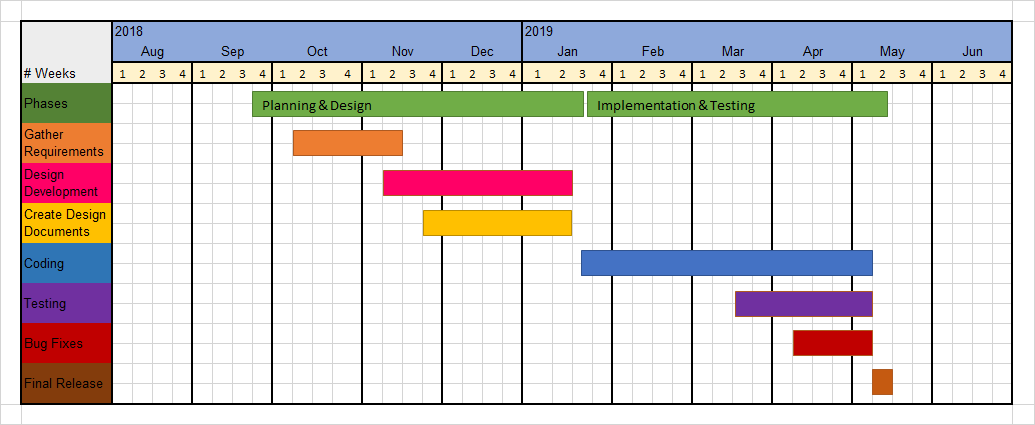
\includegraphics[width=\linewidth]{./gantt.png}
     \end{figure}
     
     \subsection{Document Revisions made}
\begin{tabular}{ |p{5cm}|p{5cm}|p{5cm}|  }
 \hline
 \multicolumn{3}{| c |}{Changes made to the original document} \\
 \hline
 Section  &  Original  &  New\\
 \hline
 2.1 Functional Requirements &
 \begin{itemize}
  \item FR3 - JSON editing
  \item FR4 - Adding and removing JSON elements
  \item FR5 - Time-line integration
\end{itemize}
 &   \begin{itemize}
  \item Removed FR3 - JSON editing
  \item Removed FR4 - Adding and removing JSON elements
  \item Removed FR5 - Time-line integration
  \item Added Filtering functionality (the new FR3)
  
\end{itemize} \\
 \hline
 2.2 Usability Requirements& UR2 - Pre-render element editing & Removed that requirement   \\
 \hline
 2.4 System Interface& The JSON elements could be individually added/removed/edited. & The JSON elements cannot  be individually added/removed/edited. \\
 \hline
3 Assumptions and Dependencies & The user can download a GIF or MOV file using the export functionality. & The user can download JPEG  image using the export functionality.\\
 \hline


    
 \hline
\end{tabular}

 
\newpage  
\newpage  
% bibliography
\nocite{*}%if nothing is referenced it will still show up in refs
\bibliographystyle{IEEEtran}
\bibliography{IEEEabrv,References.bib}



\end{document}